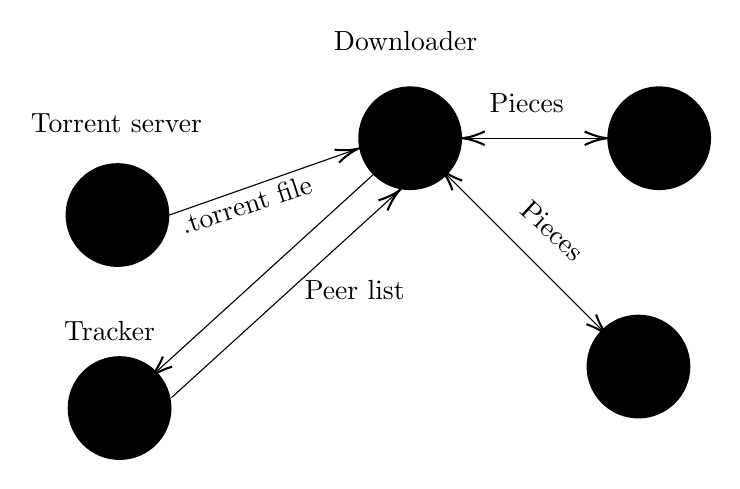
\begin{tikzpicture}[x=0.75pt,y=0.75pt,yscale=-1,xscale=1]
%uncomment if require: \path (0,300); %set diagram left start at 0, and has height of 300

%Shape: Circle [id:dp48020129375115905]
    \draw  [draw opacity=0][fill={rgb, 255:red, 0; green, 0; blue, 0 }  ,fill opacity=1 ] (290,195) .. controls (290,181.19) and (301.19,170) .. (315,170) .. controls (328.81,170) and (340,181.19) .. (340,195) .. controls (340,208.81) and (328.81,220) .. (315,220) .. controls (301.19,220) and (290,208.81) .. (290,195) -- cycle ;
%Shape: Circle [id:dp34478913628095786]
    \draw  [draw opacity=0][fill={rgb, 255:red, 0; green, 0; blue, 0 }  ,fill opacity=1 ] (289,102) .. controls (289,88.19) and (300.19,77) .. (314,77) .. controls (327.81,77) and (339,88.19) .. (339,102) .. controls (339,115.81) and (327.81,127) .. (314,127) .. controls (300.19,127) and (289,115.81) .. (289,102) -- cycle ;
%Shape: Circle [id:dp057127662756395914]
    \draw  [draw opacity=0][fill={rgb, 255:red, 0; green, 0; blue, 0 }  ,fill opacity=1 ] (430,65) .. controls (430,51.19) and (441.19,40) .. (455,40) .. controls (468.81,40) and (480,51.19) .. (480,65) .. controls (480,78.81) and (468.81,90) .. (455,90) .. controls (441.19,90) and (430,78.81) .. (430,65) -- cycle ;
%Shape: Circle [id:dp4152860206319915]
    \draw  [draw opacity=0][fill={rgb, 255:red, 0; green, 0; blue, 0 }  ,fill opacity=1 ] (550,65) .. controls (550,51.19) and (561.19,40) .. (575,40) .. controls (588.81,40) and (600,51.19) .. (600,65) .. controls (600,78.81) and (588.81,90) .. (575,90) .. controls (561.19,90) and (550,78.81) .. (550,65) -- cycle ;
%Shape: Circle [id:dp7865484354927322]
    \draw  [draw opacity=0][fill={rgb, 255:red, 0; green, 0; blue, 0 }  ,fill opacity=1 ] (540,175) .. controls (540,161.19) and (551.19,150) .. (565,150) .. controls (578.81,150) and (590,161.19) .. (590,175) .. controls (590,188.81) and (578.81,200) .. (565,200) .. controls (551.19,200) and (540,188.81) .. (540,175) -- cycle ;
%Straight Lines [id:da837231546510533]
    \draw    (339,102) -- (428.11,70.66) ;
    \draw [shift={(430,70)}, rotate = 160.63] [color={rgb, 255:red, 0; green, 0; blue, 0 }  ][line width=0.75]    (10.93,-3.29) .. controls (6.95,-1.4) and (3.31,-0.3) .. (0,0) .. controls (3.31,0.3) and (6.95,1.4) .. (10.93,3.29)   ;
%Straight Lines [id:da29190602799399223]
    \draw    (440,80) -- (331.48,178.65) ;
    \draw [shift={(330,180)}, rotate = 317.73] [color={rgb, 255:red, 0; green, 0; blue, 0 }  ][line width=0.75]    (10.93,-3.29) .. controls (6.95,-1.4) and (3.31,-0.3) .. (0,0) .. controls (3.31,0.3) and (6.95,1.4) .. (10.93,3.29)   ;
%Straight Lines [id:da7788788491503738]
    \draw    (340,190) -- (448.52,91.35) ;
    \draw [shift={(450,90)}, rotate = 137.73] [color={rgb, 255:red, 0; green, 0; blue, 0 }  ][line width=0.75]    (10.93,-3.29) .. controls (6.95,-1.4) and (3.31,-0.3) .. (0,0) .. controls (3.31,0.3) and (6.95,1.4) .. (10.93,3.29)   ;
%Straight Lines [id:da42573370946311306]
    \draw    (548,65) -- (482,65) ;
    \draw [shift={(480,65)}, rotate = 360] [color={rgb, 255:red, 0; green, 0; blue, 0 }  ][line width=0.75]    (10.93,-3.29) .. controls (6.95,-1.4) and (3.31,-0.3) .. (0,0) .. controls (3.31,0.3) and (6.95,1.4) .. (10.93,3.29)   ;
    \draw [shift={(550,65)}, rotate = 180] [color={rgb, 255:red, 0; green, 0; blue, 0 }  ][line width=0.75]    (10.93,-3.29) .. controls (6.95,-1.4) and (3.31,-0.3) .. (0,0) .. controls (3.31,0.3) and (6.95,1.4) .. (10.93,3.29)   ;
%Straight Lines [id:da47394536708390655]
    \draw    (548.59,158.59) -- (471.41,81.41) ;
    \draw [shift={(470,80)}, rotate = 45] [color={rgb, 255:red, 0; green, 0; blue, 0 }  ][line width=0.75]    (10.93,-3.29) .. controls (6.95,-1.4) and (3.31,-0.3) .. (0,0) .. controls (3.31,0.3) and (6.95,1.4) .. (10.93,3.29)   ;
    \draw [shift={(550,160)}, rotate = 225] [color={rgb, 255:red, 0; green, 0; blue, 0 }  ][line width=0.75]    (10.93,-3.29) .. controls (6.95,-1.4) and (3.31,-0.3) .. (0,0) .. controls (3.31,0.3) and (6.95,1.4) .. (10.93,3.29)   ;

% Text Node
    \draw (271,52) node [anchor=north west][inner sep=0.75pt]   [align=left] {Torrent server};
% Text Node
    \draw (287,152) node [anchor=north west][inner sep=0.75pt]   [align=left] {Tracker };
% Text Node
    \draw (417,12) node [anchor=north west][inner sep=0.75pt]   [align=left] {Downloader};
% Text Node
    \draw (341.71,101.92) node [anchor=north west][inner sep=0.75pt]  [rotate=-341.81] [align=left] {.torrent file};
% Text Node
    \draw (403,132) node [anchor=north west][inner sep=0.75pt]   [align=left] {Peer list};
% Text Node
    \draw (492,42) node [anchor=north west][inner sep=0.75pt]   [align=left] {Pieces};
% Text Node
    \draw (513.44,92.15) node [anchor=north west][inner sep=0.75pt]  [rotate=-42.84] [align=left] {Pieces};

\end{tikzpicture}

